\section{Einleitung}

Diese Ausarbeitung ist neben dem produzierten Quellcode das Resultat des
Master Informatik Teamprojekts von \autor im Sommersemester 2013 bis
Wintersemester 2013/2014.

Es geht darum den visuellen Editor der durch Spray generiert wird
von Eclipse Graphiti ins Web zu bringen, also mit den Webtechnologien
HTML, CSS, JavaScript und einer Webservertechnologie.
Spray soll also später in der Lage sein, auch genau diesen Spray
Web Editor zu generieren (parallel zu dem gewöhnlichen Graphiti Editor).

Sämtlicher Quellcode ist im Git-Repositorium
tprj-msi-ss13\footnote{Github Link: \url{TODO}} zu finden.
Es gliedert sich in:

\begin{itemize}
  \item {\tt archive} \\
  Hier befindet sich alter Code, der hauptsächlich aus Experimenten besteht.
  Aus diesem Code ist zum Großteil der Produktionscode hervorgegangen,
  könnte aber noch nützlich sein für künftige Weiterentwicklungen.
  \item {\tt docs} \\
  Der Quellcode dieser Dokumentation als LaTeX bzw. XeLaTeX Code.
  \item {\tt generators} \\
  Dort befinden sich die Generatoren um Shapes und Spray-Logik in JSON umzuwandeln.
  \item {\tt server} \\
  Der komplette lauffähige Produktions-Code.
  Ein {\tt play 2.2.1} Server stellt anhand der beispielhaft vorgegebenen
  Spray-Defintionen den Spray Web Editor dar.
  \begin{itemize}
    \item {\tt public/javascripts/spray} \\
    Der Hauptteil des Spray Web Editors (JavaScript Code).
    \item {\tt app/controllers} \\
    Hauptanwendung von Spray, stellt insbesondere einen WebSocket sowie die
    Persistierung des vom Editor erstellten Modells bereit.
    \item {\tt app/views} \\
    Hier werden alle Spray Web Editor Komponenten als HTML-Tempaltes zusammengebracht.
  \end{itemize}
\end{itemize}

\noindent Wenn das Playframework in Version 2.2.1 installiert ist,
kann der Server wie folgt gestartet werden:

\begin{verbatim}
git clone TODO
cd tprj-msi-ss13/server
play run
\end{verbatim}

\noindent Danach kann die Webseite mit dem Spray Web Editor im
Webbrowser\footnote{Getestet mit Google Chrome 32.x, Apple Safari 7.x oder Mozilla Firefox 26.x unter Windows 7 bzw. Mac OS X 10.9.}
auf \url{http://localhost:9000/} betrachtet werden.


\subsection{Einführung in Spray}

\begin{quote}
The Graphiti framework is a new approach to create highly sophisticated
visual editors on top of the GEF framework.
Graphiti can easily be integrated with EMF as the
domain modeling framework. [...]
Spray aims to provide Domain Specific Languages (DSL) [...]
to describe Visual DSL Editors [...]
and provide code generation [...] to create the boilerplate code
for [...] the Graphiti framework. [...]
With the help of the tools created with Spray,
Graphiti based diagram editors can be created much faster
and reliable than doing it purely by hand. \citep{sprayWebpage}
\end{quote}

\noindent Das bedeutet: Spray bietet domänenspezifische Sprachen (DSLs) an,
um einen grafischen Editor zu beschreiben. Man könnte sagen, dass
man mit Spray eine Grammatik für grafische Editoren an die Hand bekommt.
Man beschreibt textuell das Layout und Aussehen von Shapes, und beschreibt
zudem was zulässige Verbindungen zwischen den einzelnen Shapes sind.
Resultat ist ein domänenspezifischer grafischer Editor.
Auf Abbildung \ref{fig.sprayArchi} ist der prinzipelle Spray zu Editor Ablauf. 

\begin{figure}[h!]
  \centering
  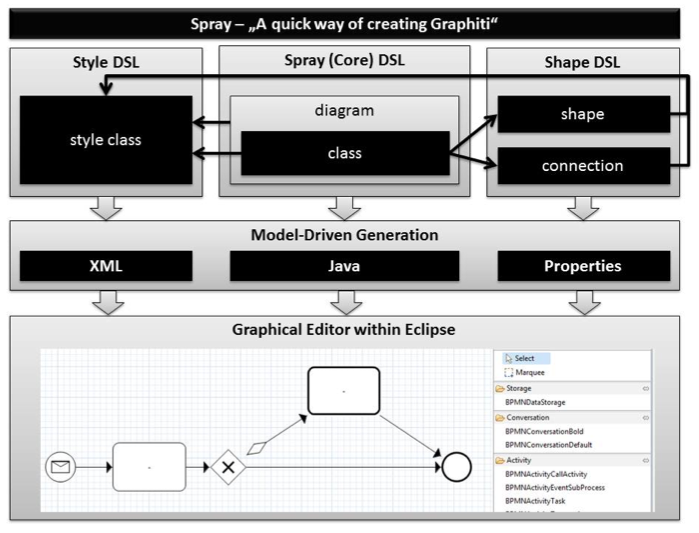
\includegraphics[width=1.0\textwidth]{Figures/SprayArchitektur.png}
  \caption{Prinzipelle Architektur von Spray. \citep[aus][S.~3]{sprayPaper}}\label{fig.sprayArchi}
\end{figure}


\subsection{Ziele von „Spray Web“}

Die Hauptaufgabe dieses Projekts ist herauszufinden, wie man diese
Editoren möglichst generisch mit Webtechnologie umsetzen kann.
Dazu gehört, dass die Shapes sowie Connections nach den von Spray
vorgegebenen (Layout) Definitionen dargestellt werden können.

Spray gibt auch (Logik) Definitionen vor,
was für Shapes miteinander über welche Connection verbunden werden darf.
Es sollte also über den Edior abgefangen werden können, wenn versucht wird
falsche Connections zu knüpfen.

Aus den Shapes und deren Connections entsteht ein konkretes Modell,
welches vom Benutzer so modelliert wurde. Dieses Modell ist die Instanz
des darüberliegenden Metamodells.
Das Metamodell entsteht also implizit aus den druch Spray vorgegebene
Logikdefinitionen. Genauer gesagt ensteht ein Ecore Metamodell,
dazu mehr im Abschnitt \ref{sec.ecore}.
Diese Modellinstanz entsteht aus dem was der Benutzer „zusammenklickt“,
dies muss durch den Web Editor ebenfalls persisiert werden.

Dieses Teamprojekt ist als Forschungsarbeit zu verstehen
auf deren Erkenntnisse und Fundamente aufgesetzt werden kann.
Die Hauptziele zusammengefasst sind:

\begin{itemize}
  \item Shapes gemäß den Definitionen produzieren,
  \item Modellüberprüfung auf Korrektheit,
  \item Persistierung der Modellinstanz (sowie Koordinaten der gesetzten Shapes).
\end{itemize}


\subsection{Ecore Metamodell}\label{sec.ecore}

\subsection{Graphiti}


\section{Anforderungen}

\subsection{Primitive Shapes}

\subsection{Connections}

\subsection{Compartments}

\subsection{Generalisierbarkeit}


\section{Architektur}


\section{Umsetzung}


\subsection{Shapes zeichnen}

\subsubsection{Toolkits}

\subsubsection{\dd}

\citep{dd}

\subsubsection{Shape Factory}

Rekursives Zeichnen der Shapes aus einer Definition

\subsubsection{Compartments}


\subsection{Code-Generierung}

\subsubsection{Shape Layout Definitionen}

\subsubsection{Spray Logik Definitionen}

Definitionen für ein zulässiges Modell.

\subsection{Validierung und Persistierung}

\subsubsection{Anwendung der abgeleiteten Modell Regeln}

Regeln abgeleitet aus dem Modell mit \dd abfangen.

\subsubsection{EMF REST}

\subsubsection{Ecore.js}

\subsubsection{Ecore mit Server}


\section{Nächste Ausbaustufen}

\subsection{Alternative Zeichentoolkits}

go.js oder digaram.js sind eleganter?
Unsere bisherigen Erkenntnisse einbringen.

\subsection{Pflege Codebasis}

Bisheriges verbessern, stabilisieren und testen.

\subsection{Kollobarationsfähigkeit}

\subsection{Validierung ausbauen}

Gibt es andere Möglichkeiten zu validieren oder zu persistieren?
Reine Client-Validierung, also Standalone im Browser oder doch Server?

\subsection{Spray Integration}

Den bisherigen Code in Spray vernünftige integrieren, mit Tests, sowie
den Dev und User Guide entsprechend erweitern.
Generator der Spray Grammatik übersetzt auf die neue Grammatik von Thomas u.a.
portieren?


\section{Zusammenfassung}

Fazi und Zusammenfassung der Ergebnisse.
